%-------------------------------------------------------------------------------
%-------------------------------------------------------------------------------
%-------------------------------------------------------------------------------
\chapter{SQL : jointures}
%-------------------------------------------------------------------------------
%-------------------------------------------------------------------------------
\thispagestyle{empty}
%-------------------------------------------------------------------------------
%-------------------------------------------------------------------------------
\vskip -2cm
%--------------------------------------------------------------------------
%--------------------------------------------------------------------------
\section{Introduction}
%--------------------------------------------------------------------------
%--------------------------------------------------------------------------
%--------------------------------------------------------------------------
Nous allons utiliser une base de données concernant les films.

Les données sont issues d'un projet collaboratif, IMDb (internet movie database).

Pour des raisons de taille la base est restreinte aux films sortis avant 1950.

Elle est composée de 5 tables.

\begin{center}
\tikzstyle{table}=[draw,shape=rectangle,text width=28mm,align=center,minimum height=6mm]
\tikzpicture
\node[table] at (-1, 1.0) {\bf personnes};
\node[table] at (-1, 0.4) (id-p) {id};
\node[table] at (-1,-0.2) {Nom};
\node[table] at (-1,-0.8) {Naissance};
\node[table] at (-1,-1.4) {Deces};
\node[table] at (4, 3.0) {\bf filmsActeurs};
\node[table] at (4, 2.4) (id-f-ac) {id\_film};
\node[table] at (4, 1.8) (id-p-ac) {id\_acteur};
\node[table] at (4, 1.2) {Role};
\node[table] at (4, 0.3) {\bf filmsAuteurs};
\node[table] at (4,-0.3) (id-f-au) {id\_film};
\node[table] at (4,-0.9) (id-p-au) {id\_auteur};
\node[table] at (4,-1.8) {\bf filmsReal};
\node[table] at (4,-2.4) (id-f-r) {id\_film};
\node[table] at (4,-3.0) (id-p-r) {id\_real};
\draw[thick, <->] (id-p) -- +(3,0) |- (id-p-ac);
\draw[thick, <->] (id-p) -- +(2.5,0) |- (id-p-au);
\draw[thick, <->] (id-p) -- +(2,0) |- (id-p-r);
\node[table] at ( 9, 1.0) {\bf films};
\node[table] at ( 9, 0.4) (id-f) {id};
\node[table] at ( 9,-0.2) {Titre};
\node[table] at ( 9,-0.8) {Annee};
\node[table] at ( 9,-1.4) {Genre};
\draw[thick, <->] (id-p) -- +(3,0) |- (id-p-ac);
\draw[thick, <->] (id-p) -- +(2.5,0) |- (id-p-au);
\draw[thick, <->] (id-p) -- +(2,0) |- (id-p-r);
\draw[thick, <->] (id-f) -- +(-3,0) |- (id-f-ac);
\draw[thick, <->] (id-f) -- +(-2.5,0) |- (id-f-au);
\draw[thick, <->] (id-f) -- +(-2,0) |- (id-f-r);
\endtikzpicture
\end{center}

\begin{itemize}
  \item {\bf films}, qui donne des renseignements sur les films.
  
    \type{id} : un identifiant unique de chaque film
    
    \type{Titre} : le titre du film
   
   \type{Annee} : l'année de sortie du film
   
   \type{Genre} : le genre du film
 
  \item {\bf personnes}, qui donne des renseignement sur ceux qui ont travaillé sur le film
  
  \type{id} : un identifiant unique de chaque personne
  
  \type{Nom} : le prénom et le nom
  
  \type{Naissance} : l'année de naissance
  
  \type{Deces} : l'année de décès (-1 si la personne est en vie)

  \item {\bf filmsActeurs}, qui indique les acteurs principaux d'un film

   \type{id\_film} : l'identifiant du film
   
   \type{id\_acteur} : l'identifiant de l'acteur
   
   \type{Role} : le rôle joué par l'acteur

\item {\bf filmsAuteurs}, qui indique les auteurs d'un film

  \type{id\_film} : l'identifiant du film
  
  \type{id\_acteur} : l'identifiant de l'auteur

  \item {\bf filmsReal}, qui indique le(s) réalisateur(s) d'un film

  \type{id\_film} : l'identifiant du film
  
  \type{id\_real} : l'identifiant du réalisateur
\end{itemize}

\begin{enumerate}
  \item Les tables {\bf films} et  {\bf personnes} sont des tables d'{\it entités}, elles décrivent des personnes ou des objets. On peut ajouter des caractéristiques au fur et à mesure que l'on en a connaissance.
  \item Les tables {\bf filmsActeurs}, {\bf filmsAuteurs} et {\bf filmsReal} sont des tables de {\it relations}, elles associent des entités.
  \item On a regroupé les descriptions des auteurs, acteurs et réalisateurs dans une même table ; les caractéristiques sont indépendantes des actions qu'ils peuvent réaliser. Une même personne peut d'ailleurs intervenir de différentes façons.
  \item Les égalités d'identifiants symbolisées par les flèches ci-dessus sont structurelles ; elles {\bf devront} être utilisées pour faire des jointures et non dans des clauses \type{WHERE}.
  \item Même si la base de données a été réduite elle reste de grande taille : les réponses aux requêtes peuvent être longues à obtenir (de l'ordre de plusieurs secondes).
  \item Il est {\bf indispensable} de copier la base sur l'ordinateur, en local, et d'utiliser cette copie. Dans le cas contraire les requêtes auront un temps de réponse prohibitif. 
\end{enumerate}
%--------------------------------------------------------------------------
%--------------------------------------------------------------------------
\section{Rappels}
%--------------------------------------------------------------------------
%--------------------------------------------------------------------------
\subsection{Requêtes simples}
%--------------------------------------------------------------------------
%--------------------------------------------------------------------------
\begin{Exercise} \it 
Quels sont les films marqués par le genre \type{"Film-Noir"} ? (Il y en a 28.)
\end{Exercise}
%--------------------------------------------------------------------------
\begin{Answer}
\begin{lstlisting}[language=SQL]
select Titre
from films
where Genre = "Film-Noir"
\end{lstlisting}
\end{Answer}
%--------------------------------------------------------------------------
%--------------------------------------------------------------------------
\begin{Exercise} \it 
Quelles sont les personnes répertoriées qui sont nées avant 1500 ? (Il y en a 10.)

On peut remarquer une erreur de la table si on demande l'année de décès.
\end{Exercise}
%--------------------------------------------------------------------------
\begin{Answer}
\begin{lstlisting}[language=SQL]
select Nom, Naissance, Deces
from personnes
where Naissance < 1500
\end{lstlisting}
Ovide est marqué comme encore vivant.
\end{Answer}
%--------------------------------------------------------------------------
%--------------------------------------------------------------------------
\begin{Exercise} \it Quels sont les films dont le titre contient Sherlock Holmes ? (Il y en a 18.)

\type{like} pour la ressemblance, \% pour une chaîne quelconque.
\end{Exercise}
%--------------------------------------------------------------------------
\begin{Answer}
\begin{lstlisting}[language=SQL]
select Titre
from films
where Titre like "%Sherlock Holmes%"
\end{lstlisting}
\end{Answer}
%--------------------------------------------------------------------------
%--------------------------------------------------------------------------
\begin{Exercise} \it Quels sont les films dont le titre contient le mot "Napoleon"  ? Il y en a 16.
\end{Exercise}
%--------------------------------------------------------------------------
\begin{Answer}
\begin{lstlisting}[language=SQL]
select titre
from films 
where titre like "%Napoleon%" 
\end{lstlisting}
\end{Answer}
%--------------------------------------------------------------------------
%--------------------------------------------------------------------------
\subsection{Agrégations} 
%--------------------------------------------------------------------------
%--------------------------------------------------------------------------
\begin{Exercise} \it 
Combien y-a-t-il de films par année ?

\type{sqlitebrowser} permet de visualiser le résultat graphiquement : dans le menu \type{Vue}, activer \type{Graphique}. Dans l'onglet \type{graphique} on peut sélectionner {\bf x} et {\bf y} avec les attributs utiles.
\end{Exercise}
%--------------------------------------------------------------------------
\begin{Answer}
\begin{lstlisting}[language=SQL]
select annee, count() as nombre
from films
group by annee
\end{lstlisting}
\end{Answer}
%--------------------------------------------------------------------------
%--------------------------------------------------------------------------
\begin{center}
    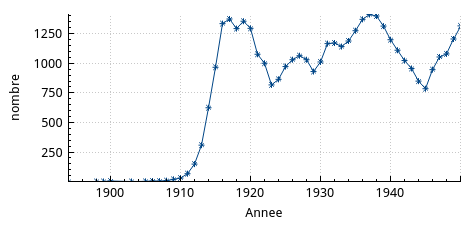
\includegraphics[width = 8cm]{Jointures_filmsAnnees}
  \end{center}
%--------------------------------------------------------------------------
%--------------------------------------------------------------------------
\begin{Exercise} \it 
Combien y-a-t-il de films par genre ?
\end{Exercise}
%--------------------------------------------------------------------------
\begin{Answer}
\begin{lstlisting}[language=SQL]
select genre, count() as nombre
from films
group by genre
\end{lstlisting}
\end{Answer}
%--------------------------------------------------------------------------
%--------------------------------------------------------------------------
\begin{Exercise} \it Quels sont les titres qui sont partagés par le plus de films ? 

2 titres sont partagés par 9 films.
\end{Exercise}
%--------------------------------------------------------------------------
\begin{Answer}
\begin{lstlisting}[language=SQL]
Select Titre, Count() as nb
From Films
Group by Titre
Order by nb desc
\end{lstlisting}
\newpage
\end{Answer}
%--------------------------------------------------------------------------
%--------------------------------------------------------------------------
\begin{Exercise} \it Écrire une requête qui donne uniquement les titres qui réalisent le maximum.
\end{Exercise}
%--------------------------------------------------------------------------
\begin{Answer}
\begin{lstlisting}[language=SQL]
Select Titre, nb
From (Select Titre, Count() as nb From Films Group by Titre)
where nb = (Select Max(nb) 
            From (Select Titre, Count() as nb 
                  From Films 
                  Group by Titre))
\end{lstlisting}
\end{Answer}
%--------------------------------------------------------------------------
%--------------------------------------------------------------------------
\section{Jointures de deux tables}
%--------------------------------------------------------------------------
%--------------------------------------------------------------------------
\subsection{Jointures simples}
%--------------------------------------------------------------------------
%--------------------------------------------------------------------------
\begin{Exercise} \it 
Quels sont les rôles joués dans le Magicien d'Oz ("The Wizard of Oz") ? Il y en a 4. 
\end{Exercise}
%--------------------------------------------------------------------------
\begin{Answer}
\begin{lstlisting}[language=SQL]
select fa.Role
from films as f join filmsActeurs as fa on f.id = fa.id_film
where f.Titre = "The Wizard of Oz"
\end{lstlisting}
\end{Answer}
%--------------------------------------------------------------------------
%--------------------------------------------------------------------------
\begin{Exercise} \it Quels sont les films dans lesquels un personnage a un nom qui contient "Napoleon" (dans la base les noms n'ont pas d'accent) ? 
Il y en a 34.
\end{Exercise}
%--------------------------------------------------------------------------
\begin{Answer}
\begin{lstlisting}[language=SQL]
select distinct f.titre
from films as f join filmsActeurs as fa on f.id = fa.id_film
where fa.role like "%Napoleon%" 
\end{lstlisting}
\end{Answer}
%--------------------------------------------------------------------------
%--------------------------------------------------------------------------
\begin{Exercise} \it Quels sont les films dans lesquels un personnage a un nom qui contient "Napoleon" (dans la base les noms n'ont pas d'accent) ? 
Il y en a 33.
\end{Exercise}
%--------------------------------------------------------------------------
\begin{Answer}
\begin{lstlisting}[language=SQL]
select distinct f.titre
from films as f join filmsActeurs as fa on f.id = fa.id_film
where fa.role like "%Napoleon%" 
\end{lstlisting}
\end{Answer}
%--------------------------------------------------------------------------
%--------------------------------------------------------------------------
\begin{Exercise} \it Quels sont les acteurs qui ont joué Sherlock Holmes ? 

Il y en a 17 distincts.
\end{Exercise}
%--------------------------------------------------------------------------
\begin{Answer}
\begin{lstlisting}[language=SQL]
select distinct p.nom
from filmsActeurs as fa join personnes as p on p.id = fa.id_acteur
where fa.Role = "Sherlock Holmes"
\end{lstlisting}
\end{Answer}
%--------------------------------------------------------------------------
%--------------------------------------------------------------------------
\begin{Exercise} \it Quels sont les acteurs ayant joué au moins un rôle contenant le mot "Sheriff" ? 

Il y en a 254 distincts.
\end{Exercise}
%--------------------------------------------------------------------------
\begin{Answer}
\begin{lstlisting}[language=SQL]
select distinct p.nom, fa.role
from filmsActeurs as fa join personnes as p on p.id = fa.id_acteur
where fa.Role like "%heriff%"
\end{lstlisting}
\end{Answer}
%--------------------------------------------------------------------------
%--------------------------------------------------------------------------
\begin{Exercise} \it Quels sont les films dont le titre contient le mot "Napoleon" mais pour lesquels n'est pas indiqué de personnage dont le nom contient "Napoleon" ou qui n'ont pas de personnage indiqué ? Il y en a 10.
\end{Exercise}
%--------------------------------------------------------------------------
\begin{Answer}
\begin{lstlisting}[language=SQL]
select titre
from films 
where titre like "%Napoleon%" 
EXCEPT
select distinct f.titre
from films as f join filmsActeurs as fa on f.id = fa.id_film
where fa.role like "%Napoleon%" 
\end{lstlisting}
\newpage
\end{Answer}
%--------------------------------------------------------------------------
%--------------------------------------------------------------------------
\subsection{Jointures avec agrégations}
%--------------------------------------------------------------------------
%--------------------------------------------------------------------------
\begin{Exercise} \it Un acteur a joué le rôle de Sherlock Holmes plus de 10 fois ; qui est-il ? 
\end{Exercise}
%--------------------------------------------------------------------------
\begin{Answer}
\begin{lstlisting}[language=SQL]
select distinct p.nom, count() as nombre
from filmsActeurs as fa join personnes as p on p.id = fa.id_acteur
where fa.Role = "Sherlock Holmes"
group by p.nom
having nombre >= 10
\end{lstlisting}

C'est Basil Rathbone.
\end{Answer}
%--------------------------------------------------------------------------
%--------------------------------------------------------------------------
\begin{Exercise} \it Déterminer, pour chaque année, le nombre d'acteurs ayant joué dans au moins un film. Pour compter le nombre d'acteurs et non le nombre de rôles joués on pourra utiliser
\type{COUNT(DISTINCT filmsActeurs.id\_acteur)}
\end{Exercise}
%--------------------------------------------------------------------------
\begin{Answer}
\begin{lstlisting}[language=SQL]
select f.Annee, count(distinct fa.id_acteur) as nb
from films as f join filmsActeurs as fa on fa.id_film = f.id
group by f.annee
\end{lstlisting}
\begin{center}
    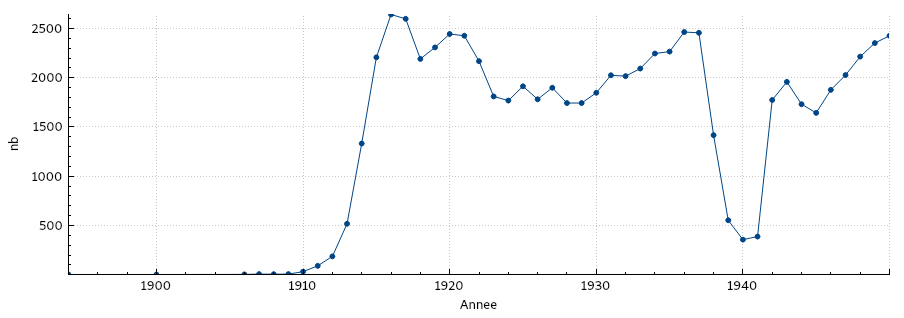
\includegraphics[width = 12cm]{Jointures_acteurs_annee}
  \end{center}
  \end{Answer}
%--------------------------------------------------------------------------
%--------------------------------------------------------------------------
\begin{Exercise} \it Parfois des acteurs jouent des rôles avec leur vrai nom. 

Quels acteurs on ainsi joué dans plus de 20 films en portant leur nom ? Il y en a 3.
\end{Exercise}
%--------------------------------------------------------------------------
\begin{Answer}
\begin{lstlisting}[language=SQL]
select distinct p.nom, count() as nombre
from filmsActeurs as fa join personnes as p on p.id = fa.id_acteur
where fa.Role = p.nom
group by p.nom
having nombre > 20
\end{lstlisting}
\end{Answer}
%--------------------------------------------------------------------------
%--------------------------------------------------------------------------
\begin{Exercise}[label = qu:centfilms] \it Quels sont les réalisateurs crédités de plus de 100 films dans la base ? Il y en a 17.
\end{Exercise}
%--------------------------------------------------------------------------
\begin{Answer}
\begin{lstlisting}[language=SQL]
select p.nom, count() as nombre
from personnes as p join filmsReal as fr on p.id = fr.id_real
group by p.nom
having nombre > 100
\end{lstlisting}
\end{Answer}
%--------------------------------------------------------------------------
%--------------------------------------------------------------------------
\begin{Exercise}[label = qu:realMax]\it Quel est le nombre maximal de films réalisés par un réalisateur en une année ? 

On ne demande pas ici le nom du réalisateur. On supposera qu'il n'y a pas d'ex-æquo.
\end{Exercise}
%--------------------------------------------------------------------------
\begin{Answer}
\begin{lstlisting}[language=SQL]
select f.annee, count() as nombre
from films as f join filmsReal as fr on f.id = fr.id_film
group by f.annee, fr.id_real
order by nombre DESC
limit 1
\end{lstlisting}
\newpage
\end{Answer}
%--------------------------------------------------------------------------
\newpage
%--------------------------------------------------------------------------
\section{Jointures de 3 tables ou plus}
%--------------------------------------------------------------------------
%--------------------------------------------------------------------------
Dans la structure entités-relations on voit que les entités sont séparées par une relation (au moins). Si on veut lier les noms des acteurs aux titres des films on doit donc écrire une double jointure.

On peut écrire une double jointure sous une des deux formes suivantes
%--------------------------------------------------------------------------
\begin{lstlisting}[language=SQL]
table1 AS t1 JOIN table2 AS t2 ON t1.attribut1 = t2.attribut2
             JOIN table3 AS t3 ON t1.attribut3 = t3.attribut4

table1 AS t1 JOIN table2 AS t2 JOIN table3 AS t3 
             ON     t1.attribut1 = t2.attribut2 
                AND t1.attribut3 = t3.attribut4
\end{lstlisting}
%--------------------------------------------------------------------------
%--------------------------------------------------------------------------
\subsection{Requêtes sans agrégation}
%--------------------------------------------------------------------------
%--------------------------------------------------------------------------
\begin{Exercise} \it 
Quels sont les films réalisés par Abel Gance ? Il y en a 21.
\end{Exercise}
%--------------------------------------------------------------------------
\begin{Answer}
\begin{lstlisting}[language=SQL]
select Titre, Annee
from personnes as p join filmsReal as fr on p.id = fr.id_real
                    join films as f on f.id = fr.id_film
where p.nom = "Abel Gance"
\end{lstlisting}
\end{Answer}
%--------------------------------------------------------------------------
%--------------------------------------------------------------------------
\begin{Exercise} \it Quels sont les films dans lesquels a joué Ronald Reagan ? Il y en a 10.
\end{Exercise}
%--------------------------------------------------------------------------
\begin{Answer}
\begin{lstlisting}[language=SQL]
select f.titre, f.annee
from films as f join filmsActeurs as fa on f.id = fa.id_film
                join personnes as p on p.id = fa.id_acteur
where p.nom = "Ronald Reagan"
\end{lstlisting}
Si on filtre avec \type{p.nom like "\%Reagan"} on trouve deux films en plus dans lesquels joue Nancy Reagan.
\end{Answer}
%--------------------------------------------------------------------------
%--------------------------------------------------------------------------
\begin{Exercise} \it Quels sont les films dans lesquels Charles K. French a joué un rôle indiqué comme Sheriff (The Sheriff, Sheriff Nelson, ...) ? Il y en a 8
\end{Exercise}
%--------------------------------------------------------------------------
\begin{Answer}
\begin{lstlisting}[language=SQL]
select f.titre, fa.role, f.genre
from films as f join filmsActeurs as fa on f.id = fa.id_film
                join personnes as p on p.id = fa.id_acteur
where fa.role like "%Sheriff%" and p.nom = "Charles K. French"
\end{lstlisting}
\end{Answer}
%--------------------------------------------------------------------------
%--------------------------------------------------------------------------
\begin{Exercise} \it Quels sont les films dans lesquels le réalisateur joue ? Il y en a 1056.
\end{Exercise}
%--------------------------------------------------------------------------
\begin{Answer}
\begin{lstlisting}[language=SQL]
select pr.nom, f.titre
from films as f join filmsActeurs as fa on f.id = fa.id_film
                join filmsReal as fr on f.id = fr.id_film
                join personnes as pr on pr.id = fr.id_real
                join personnes as pa on pa.id = fa.id_acteur
where pr.id = pa.id
\end{lstlisting}
\end{Answer}
%--------------------------------------------------------------------------
%--------------------------------------------------------------------------
\begin{Exercise} \it Dans quels films ont joué ensemble Fred Astaire et Ginger Rogers ? Il y en a 8.
\end{Exercise}
%--------------------------------------------------------------------------
\begin{Answer}
\begin{lstlisting}[language=SQL]
select f.titre, f.annee
from films as f join filmsActeurs as fa on f.id = fa.id_film
                join  personnes as p on p.id = fa.id_acteur
where p.nom = "Fred Astaire"
INTERSECT
select f.titre, f.annee
from films as f join filmsActeurs as fa on f.id = fa.id_film
                join  personnes as p on p.id = fa.id_acteur
where p.nom = "Ginger Rogers"
\end{lstlisting}
\end{Answer}
%--------------------------------------------------------------------------
%--------------------------------------------------------------------------
\subsection{Requêtes avec agrégation}
%--------------------------------------------------------------------------
%--------------------------------------------------------------------------
\begin{Exercise} \it À la question {\bf \ref{qu:centfilms}} on peut voir que Sam Newfield est crédité de 191 films. 

Déterminer le nombre de films qu'il a réalisé par année.
\end{Exercise}
%--------------------------------------------------------------------------
\begin{Answer}
\begin{lstlisting}[language=SQL]
select Annee, count() as nombre
from personnes as p join filmsReal as fr on p.id = fr.id_real
                    join films as f on f.id = fr.id_film
where p.nom = "Sam Newfield"
group by Annee
order by Annee
\end{lstlisting}
\begin{center}
    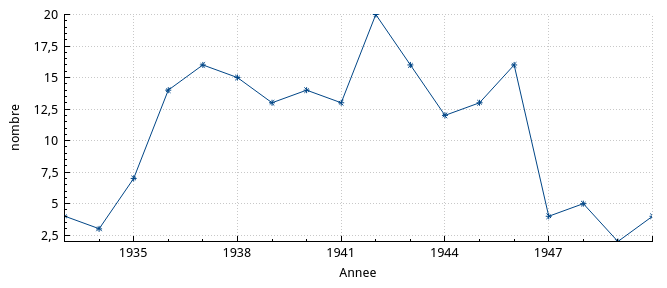
\includegraphics[width = 12cm]{Jointures_samNewfield}
  \end{center}
\end{Answer}
%--------------------------------------------------------------------------
%--------------------------------------------------------------------------
\begin{Exercise} \it Déterminer le nom du réalisateur qui a réalisé le nombre maximal de films en un an (question {\bf \ref{qu:realMax}}).
\end{Exercise}
%--------------------------------------------------------------------------
\begin{Answer}
\begin{lstlisting}[language=SQL]
select f.annee, p.nom, count() as nombre
from films as f join filmsReal as fr on f.id = fr.id_film
                join personnes as p on p.id = fr.id_real
group by f.annee, fr.id_real
order by nombre DESC
limit 1
\end{lstlisting}
\end{Answer}
%--------------------------------------------------------------------------
%--------------------------------------------------------------------------
\begin{Exercise} \it Calculer la moyenne annuelle du nombre de films réalisés par Sam Newfield entre 1936 et 1946 (limites comprises) ?
\end{Exercise}
%--------------------------------------------------------------------------
\begin{Answer}
\begin{lstlisting}[language=SQL]
select avg(nombre)
from (select Annee, count() as nombre
      from films as f join filmsReal as fr on f.id = fr.id_film
                      join personnes as p on p.id = fr.id_real
      where p.nom = "Sam Newfield"
      group by Annee)
where Annee >= 1936 and Annee <= 1946
\end{lstlisting}
\end{Answer}
%--------------------------------------------------------------------------
%--------------------------------------------------------------------------
\begin{Exercise} \it Quels sont les 3 "couples" réalisateur/acteur ayant fait le plus grand nombre de films en communs ?
\end{Exercise}
%--------------------------------------------------------------------------
\begin{Answer}
\begin{lstlisting}[language=SQL]
select pr.nom as Réal, pa.nom as Act, count(*) as "Nb films"
from filmsReal as fr join personnes as pr on fr.id_real=pr.id
            join filmsActeurs as fa on fr.id_film=fa.id_film 
            join personnes as pa on fa.id_acteur=pa.id
group by pr.id ,pa.id
order by 3 desc
limit 3
\end{lstlisting}
\newpage
\end{Answer}
%--------------------------------------------------------------------------
%--------------------------------------------------------------------------
\begin{Exercise}[difficulty = 2] \it Quels sont les "couples" réalisateur/acteur ayant fait les 4 plus grands nombres de films en communs ?
On veut tous les ex-æquo (ils sont 4) pour la quatrième position.
\end{Exercise}
%--------------------------------------------------------------------------
\begin{Answer}
\begin{lstlisting}[language=SQL]
select pr.nom as Réal, pa.nom as Act, count(*) as "Nb films"
from filmsReal as fr join personnes as pr on fr.id_real=pr.id
            join filmsActeurs as fa on fr.id_film=fa.id_film 
            join personnes as pa on fa.id_acteur=pa.id
group by pr.id ,pa.id
having count() >= (select distinct count()
                   from filmsActeurs as fa 
                           join filmsReal as fr 
                           on fr.id_film=fa.id_film 
                   group by fr.id_real,fa.id_acteur				   
                   order by 1 desc  limit 1  offset 3)
order by 3 desc
\end{lstlisting}
\end{Answer}
%--------------------------------------------------------------------------
%--------------------------------------------------------------------------
\begin{Exercise}[difficulty = 2] \it Déterminer l'acteur (ou les acteurs en cas d'ex-æquos) qui a joué le plus de films chaque année.
\end{Exercise}
%--------------------------------------------------------------------------
\begin{Answer}
\begin{lstlisting}[language=SQL]
select m.an, n.nom, m.nmax
from (select an, max(nb) as nmax
      from (select f.annee as an, p.nom as nom, count() as nb
            from films as f join filmsActeurs as fr 
                                on f.id = fr.id_film
                            join personnes as p 
                                on p.id = fr.id_acteur
                            group by f.annee, fr.id_acteur)
	  group by an) as m
	  join (select f.annee as an, p.nom as nom, count() as nb
            from films as f join filmsActeurs as fr 
                                on f.id = fr.id_film
                            join personnes as p 
                                on p.id = fr.id_acteur
            group by f.annee, fr.id_acteur) as n
	  on m.an = n.an
where n.nb = m.nmax
\end{lstlisting}
\end{Answer}
%--------------------------------------------------------------------------
\newpage
%--------------------------------------------------------------------------
\section{Complément : championnat de France}
%--------------------------------------------------------------------------
%--------------------------------------------------------------------------
%--------------------------------------------------------------------------
Nous allons travailler avec une base de données qui recense les renseignements sur les matchs de division 1 d'une année.
La base ne contient qu'une table, nommée \type{statFoot}.

\medskip

En voici quelques lignes, la saison est 2020-21
\begin{center}
\begin{tabular}{|c|c|c|c|c|c|c|c|c|}
\hline
jour        &equD       &equE       &butsD  &butsE \\
\hline
21/08/2020	&Bordeaux	&Nantes	    &0	    &0\\
22/08/2020	&Dijon	    &Angers	    &0	    &1\\
22/08/2020	&Lille	    &Rennes	    &1	    &1\\
23/08/2020	&Monaco	    &Reims	    &2	    &2\\
23/08/2020	&Lorient	&Strasbourg	&3	    &1\\
23/08/2020	&Nimes	    &Brest	    &4	    &0\\
\dots       &\dots      &\dots      &\dots  &\dots \\   
\end{tabular}
\end{center}
Il y a 20 équipes ; chaque équipe reçoit toutes les autres une fois et une seule.

\begin{itemize}
\item \type{jour} est la date du match, sous forme d'une chaîne de caractères.
\item Les autres attributs vont par paire : le suffixe \type{D} indique que l'attribut concerne l'équipe qui joue à domicile, le suffixe \type{E} indique que l'attribut concerne l'équipe qui joue à l'extérieur.
\item \type{equD} ou \type{equE} indique le nom de l'équipe, sous forme d'une chaîne de caractères.
\item \type{butsD} ou \type{butsE} indique le nombre de buts marqués pendant le match.
\end{itemize}

%--------------------------------------------------------------------------
%--------------------------------------------------------------------------
\begin{Exercise}{\it 
Écrire une requête qui permet de connaître le nombre de matchs gagnés par chaque équipe et le total des points de l'année. 

Un match nul vaut 1 point, un match gagné vaut 3 points.

N.B. Bien que la base ne contienne qu'une table, la requête fait intervenir plusieurs jointures.}
\end{Exercise}
%--------------------------------------------------------------------------
\begin{Answer}
\begin{lstlisting}[language=SQL]
select d.club, (d.victoiresD + e.victoiresE) as victoires,
      (3*(d.victoiresD + e.victoiresE) + n.nuls) as points
from (select equD as club, count() as victoiresD
      from stat where butsD > butsE group by equD) as d
	 join
	 (select equE as club, count() as victoiresE
      from stat where butsD < butsE group by equE) as e
	 join
	 (select equD as club, count() as nuls
      from stat where butsD = butsE group by equD) as n
	 on e.club = d.club and e.club = n.club
order by points desc
\end{lstlisting}
\end{Answer}
%--------------------------------------------------------------------------
%--------------------------------------------------------------------------
%--------------------------------------------------------------------------
%--------------------------------------------------------------------------
